\let\negmedspace\undefined
\let\negthickspace\undefined
\documentclass[journal]{IEEEtran}
\usepackage[a5paper, margin=10mm, onecolumn]{geometry}
%\usepackage{lmodern} % Ensure lmodern is loaded for pdflatex
\usepackage{tfrupee} % Include tfrupee package

\setlength{\headheight}{1cm} % Set the height of the header box
\setlength{\headsep}{0mm}     % Set the distance between the header box and the top of the text

\usepackage{gvv-book}
\usepackage{gvv}
\usepackage{cite}
\usepackage{amsmath,amssymb,amsfonts,amsthm}
\usepackage{algorithmic}
\usepackage{graphicx}
\usepackage{textcomp}
\usepackage{xcolor}
\usepackage{txfonts}
\usepackage{listings}
\usepackage{enumitem}
\usepackage{mathtools}
\usepackage{gensymb}
\usepackage{comment}
\usepackage[breaklinks=true]{hyperref}
\usepackage{tkz-euclide} 
\usepackage{listings}
% \usepackage{gvv}                                        
\def\inputGnumericTable{}                                 
\usepackage[latin1]{inputenc}                                
\usepackage{color}                                            
\usepackage{array}                                            
\usepackage{longtable}                                       
\usepackage{calc}                                             
\usepackage{multirow}                                         
\usepackage{hhline}                                           
\usepackage{ifthen}                                           
\usepackage{lscape}
\begin{document}

\bibliographystyle{IEEEtran}
\vspace{3cm}

\title{11.16.3.15.2}
\author{EE24BTECH11019 - Dwarak A}
% \maketitle
% \newpage
% \bigskip
{\let\newpage\relax\maketitle}

\renewcommand{\thefigure}{\theenumi}
\renewcommand{\thetable}{\theenumi}
\setlength{\intextsep}{10pt} % Space between text and floats


\numberwithin{equation}{enumi}
\numberwithin{figure}{enumi}
\renewcommand{\thetable}{\theenumi}

\textbf{Question:}

If $A$ and $B$ are events such that
\begin{align}
    P\brak{A} &= 0.25 \\
    P\brak{B} &= 0.5 \\
    P\brak{AB} &= 0.125
\end{align}
Find
\begin{align}
    P\brak{A^\prime B^\prime }
\end{align}

\solution

\textbf{Theoretical Solution (Boolean Logic):}

For 2 Boolean variables $A$ and $B$, the axioms of Boolean Algebra are defined as:
\begin{align}
    A + A &= A\\
    AA &= A \\
    A + A^\prime  &= 1\\
    AA^\prime  &= 0 \\
    AB &= BA\\
    A + B &= B + A\\
    \brak{A + B} + C &= A + \brak{B + C} \\
    \brak{AB}C &= A\brak{BC} \\
    A\brak{B + C} &= AB + AC \\
    A + BC &= \brak{A + B}\brak{A + C} \\
    P\brak{1} &= 1\\
    P\brak{A + B} &= P\brak{A} + P\brak{B}, \text{ if } P\brak{AB} = 0
\end{align}

De Morgan's Theorems:
\begin{align}
    \brak{A + B}^\prime  = A^\prime  B^\prime  \label{eq:dm1} \\
    \brak{AB}^\prime  = A^\prime  + B^\prime  \label{eq:dm2}
\end{align}

Using these axioms,
\begin{align}
    A &= A\brak{B + B^\prime } \\
    &= AB + AB^\prime  \label{eq:A}\\
    B &=\brak{A+A^\prime }B \\
    &= AB + A^\prime  B \label{eq:B}\\
    P\brak{A} &= P\brak{AB} + P\brak{AB^\prime }\\
    P\brak{B} &= P\brak{AB} + P\brak{A^\prime  B}
\end{align}
On adding \eqref{eq:A} and \eqref{eq:B},
\begin{align}
    A + B &= AB + AB + AB^\prime  + A^\prime  B\\
    A + B &= AB + AB^\prime  + A^\prime  B \label{eq:A+B}\\
    P\brak{A + B} &= P\brak{AB + AB^\prime  + A^\prime  B}\\
    P\brak{A + B} &= P\brak{AB} + P\brak{AB^\prime } + P\brak{A^\prime  B}\\
    P\brak{A + B} &= P\brak{AB} + P\brak{A} - P\brak{AB} + P\brak{B} - P\brak{AB}\\
    \implies P\brak{A + B} &= P\brak{A} + P\brak{B} - P\brak{AB} \label{eq:P(A+B)}
\end{align}

Using \eqref{eq:A+B} and \eqref{eq:dm1},
\begin{align}
    \brak{A+B}^\prime  &= A^\prime B^\prime  \\
    P\brak{\brak{A+B}^\prime } &= P\brak{A^\prime B^\prime } \\
    1 - P\brak{A+B} &= P\brak{A^\prime B^\prime } \label{eq:P(A'B')}
\end{align}

Using \eqref{eq:P(A'B')} and \eqref{eq:P(A+B)},
\begin{align}
    P\brak{A^\prime B^\prime } &= 1 - \brak{P\brak{A} + P\brak{B} - P\brak{AB}} \\
    P\brak{A^\prime B^\prime } &= 1 + P\brak{AB} - P\brak{A} - P\brak{B}
\end{align}

Using the given values of $P\brak{A},\,P\brak{B}$ and $P\brak{AB}$,
\begin{align}
    P\brak{A^\prime B^\prime } &= 1 + 0.125 - 0.25 - 0.5 \\
    P\brak{A^\prime B^\prime } &= 0.375
\end{align}
Therefore, the value of $P\brak{A^\prime B^\prime }$ is $0.375$.

\textbf{Computational Solution:}\\
Let $X_1$ be an indicator random variable of the event $A$.\\
$X_1$ is defined as:
\begin{align}
	X_1 =
	\begin{cases}
		1 ,& A\\
		0 ,& A^\prime \\
	\end{cases}
\end{align}
Let $X_2$ be the indicator random variable of the event $B$.\\
$X_2$ is defined as:
\begin{align}
	X_2 =
	\begin{cases}
		1 ,& B\\
		0 ,& B^\prime \\
	\end{cases}
\end{align}
Let $X_3$ be the indicator random variable of the event $AB$.\\
$X_3$ is defined as:
\begin{align}
	X_3 =
	\begin{cases}
		1 ,& AB\\
		0 ,& (AB)^\prime \\
	\end{cases}
\end{align}
The PMF of the random variable $X_1$ is:
\begin{align}
	p_{X_1}(n) =
	\begin{cases}
		p_1 ,& n = 1\\
		1 - p_1 ,& n = 0
	\end{cases}
\end{align}
The PMF of the random variable $X_2$ is:
\begin{align}
	p_{X_2}(n) =
	\begin{cases}
		p_2 ,& n = 1\\
		1 - p_2 ,& n = 0
	\end{cases}
\end{align}
The PMF of the random variable $X_3$ is:
\begin{align}
	p_{X_3}(n) =
	\begin{cases}
		p_3 ,& n = 1\\
		1 - p_3 ,& n = 0
	\end{cases}
\end{align}
where,
\begin{align}
	p_1 &= 0.25\\
	p_2 &= 0.50\\
	p_3 &= 0.125
\end{align}
Let $Y$ be the random variable which is defined as follows:
\begin{align}
	Y = 1 - X_1 - X_2 + X_3
\end{align}
But we know that $Y$ is another indicator random variable whose PMF is defined as:
\begin{align}
	p_Y(n) =
	\begin{cases}
		p ,& n = 1\\
		1 - p ,& n = 0
	\end{cases}
\end{align}
\begin{align}
	E(Y) &= E(1 - X_1 - X_2 + X_3)\\
	E(Y) &= E(1) - E(X_1) - E(X_2) + E(X_3)\\
	1.(p) + 0.(1 - p) &= 1.(1) - 1.(p_1) - 1.(p_2) + 1.(p_3)\\
	p &= 1 - p_1 - p_2 + p_3
\end{align}
Through our definition, we know that,
\begin{align}
	P(A) &= p_1\\
	P(B) &= p_2\\
	P(AB) &= p_3
\end{align}
Therefore, by comparison of the axiom
\begin{align}
	P(A^\prime B^\prime ) &= 1 - P(A) - P(B) + P(AB) \\
	P(A^\prime B^\prime ) &= 1 - 0.25 - 0.50 + 0.125 \\
	\implies P(A^\prime B^\prime ) &= 0.375
\end{align}

\begin{figure}[ht]
    \centering
    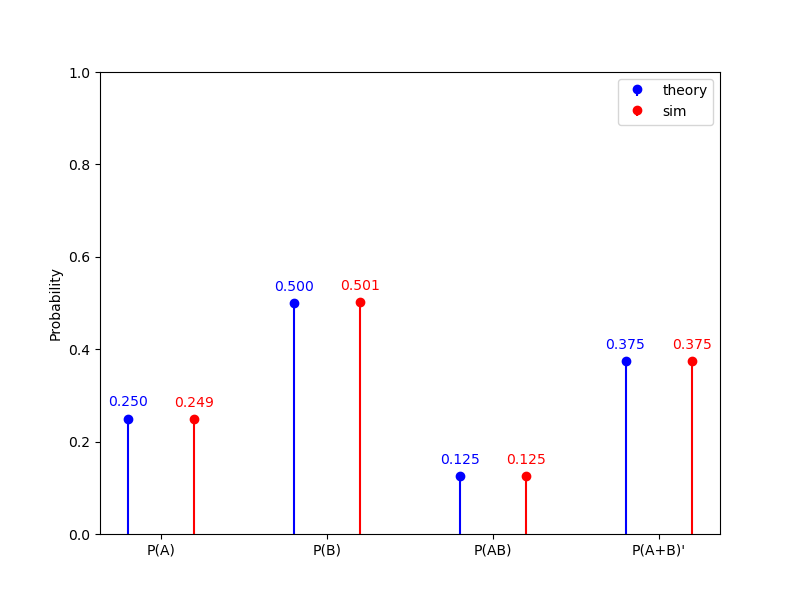
\includegraphics[width=\columnwidth]{figs/plot.png}
    \label{fig:Plot1}
\end{figure}

\end{document}
